\documentclass{standalone}
\begin{document}
\subsection{Aufgabe 13.9}
\begin{itemize}
	\item[a)] 
$\overline{W} = 2-2\sqrt{3} i$\\
$\overline{Z} = 3+i$\\
    \begin{center}
	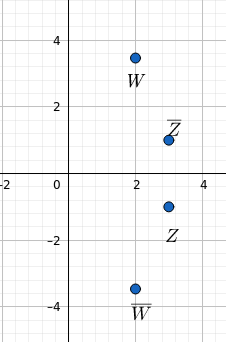
\includegraphics[width=10cm]{img/13_9_a.png}
	Die Punkten sind auf x-achse gespiegelt und die Entfernungen sind gleich.\\
\end{center}

	\item[b)]
	\begin{center}
		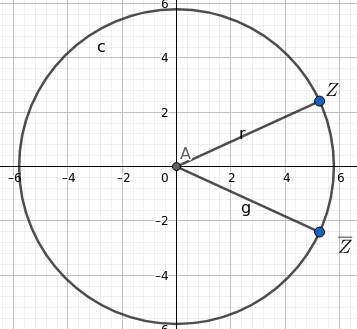
\includegraphics[width=10cm]{img/13_9_b.png}
		Die Winkel zwischen die Linen sind $2\phi$\\
	\end{center}

\end{itemize}
\subsection{Aufgabe 13.10}
\begin{itemize}
	\item[a-b)]
		\begin{center}
		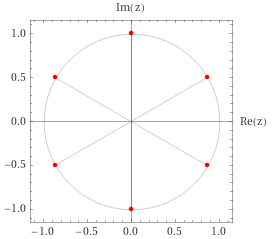
\includegraphics[width=10cm]{img/13_10.png}
		Alle lösungen befindet sich im Kreis.\\
	\end{center}
	Hier isr R=1\\
	$Z_1=exp(\frac{\pi}{2}i)=i$\\
	$Z_2=exp(\frac{3\pi}{2}i)=-i$\\
	$Z_3=exp(\frac{\pi}{6}i)=\frac{\sqrt{3}}{2}+\frac{i}{2}$\\
	$Z_4=exp(\frac{-\pi}{6}i)=\frac{\sqrt{3}}{2}-\frac{i}{2}$\\
	$Z_5=exp(\frac{5\pi}{6}i)$$=\frac{\sqrt{3}}{2}+\frac{i}{2}$\\
	$Z_6=exp(\frac{-5\pi}{6}i)$$-\frac{\sqrt{3}}{2}-\frac{i}{2}$\\
	
	\item[c)]
	\begin{center}
		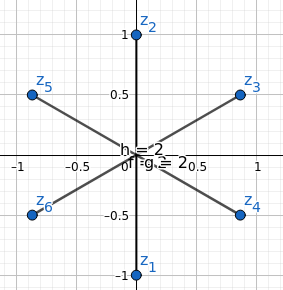
\includegraphics[width=10cm]{img/13_10_c.png}\\
		R=1\\
	\end{center}
	\item[d)] R ist hier überall geltend, also jeder Glechung ist beim Radiuskonstant vermehrt so, dass einheitsgreis der Gaussschen ebene vergrössert ist.\\	
\end{itemize}

\end{document}
